\documentclass{beamer}

\usetheme{Warsaw}
\usecolortheme{crane}
\useoutertheme{smoothbars}


\usepackage[utf8]{inputenc}
\usepackage[T1]{fontenc}
\usepackage[frenchb]{babel}
 
\title{Editeur de Livre}
\date{\today}
\author{Adama LO\\Abdou DIATTA\\Aissata CAMARA\\Mohammadou DOUCOURE}
\institute{Université de Caen Normandie}

\setbeamertemplate{navigation symbols}{}% pour enlever les symboles de navigation en bas de chaque page
\setbeamertemplate{footline}[frame number]%pour changer le pied de page par un affichage des numéros de slide

%\centering % justifier le texte
\begin{document}

\maketitle

%--------------------
\begin{frame} 
\frametitle{Plan}
\tableofcontents
\end{frame}
%--------------------
\section{\textbf{ Introduction}}

\begin{frame}
\frametitle{Introduction}
Dans le cadre de notre deuxième année de Licence Informatique  à l’Université de Caen Normandie nous avons eu pour tâche la réalisation d'un projet informatique sur le module d’enseignement nommé TPA. \\
Par groupe de quatre, il nous a été demandé de réaliser des applications complètes sur différentes thèmes: CoreWar, Simulateur pour N corps, Éditeur de livres dont vous êtes le héros, etc. Parmis ces propositions si plusieurs ont retenu notre intention, une plus que, les autres, a capté notre intérêt: \textbf{Éditeur de livres dont vous êtes le héros.}




\end{frame}
%--------------------
\begin{frame}
\subsection{Objectifs}
\frametitle{Objectifs}

 Pour chaque projet à réaliser, il y'a quelques objectifs à atteindre. Pour cela on nous a donner comme énoncé :
«Les livres dont vous êtes le héros (ou LDVEH) sont des jeux de rôles en solitaire dont la narration est décomposées en paragraphes, dispersés dans le livre. Des liens, en fonction des choix du lecteurs, permettent d’aller d’un paragraphe à l’autre. Dans un premier temps, il s’agira de développer un éditeur de texte qui maintienne le graphe du jeu et qui puisse réorganiser aléatoirement le livre. \\

\end{frame}


\begin{frame}
\frametitle{Objectifs}
 L’affichage de la ou les solutions (paragraphe devant être traversés pour gagner) devront être calculées ainsi que la difficulté du jeu (proportions de solutions au regard des chemins possibles). Dans un second temps, il s’agira d’ajouter un système de rencontres et de combat, ainsi que la gestion d’objets ou d’indices qui peuvent être nécessaire pour gagner. Enfin, un mode lecture permettant de jouer au LDVEH pourra être implanté.» 
\end{frame}

\begin{frame}
\frametitle{Objectifs}

On a trois objectifs à réaliser dans ce projet :\\

\begin{itemize}
	\item Le développement d'un éditeur de texte qui maintien le graphe du jeu et réorganise aléatoirement le livre. Le calcul de l'affichage des solutions ainsi que la difficulté du jeu.
	\item Ajouter un système de rencontres et de combat, ainsi que la gestion d’objets ou d’indices qui peuvent être nécessaire pour gagner.
	\item Un mode lecture permettant de jouer au LDVEH\footnote{LDVEH signifie «Livre dont vous êtes le héros »} pourra être implanté
\end{itemize}
\end{frame}
%--------------------
\section{\textbf{Historique}}

\begin{frame}
\frametitle{Historique}
Les livre jeux(en anglais: Gamebook), souvent appelés livre dont vous étes le héros en France et au Québec, sont un genre de romans ayant pour caracteristique d'étre interactifs, le déroulement de l'histoire dépendant des choix du lecteur.\\
Ce genre, né dans les années 1960-1970, devient célébre en 1982 avec le livre Le Sorcier de la Montagne de Feu.Le genre connaît son heure de gloire dans les années 1980 et au début des années 1990 avant de sombrer dans l'oubli,les éditeurs abandonnant la réédition de ces livres dont le succés n'est plus au rendez-vous, du fait de la concurrence des jeux vidéo.Un léger renouveau se fait sentir à partir de 2003.

\end{frame}

\begin{frame}
\frametitle{Historique}
lorsque l'éditeur anglais Wizard Books réédite les livres les plus connus de la série Défis fantastiques, suivi en 2007 par Gallimard en français. Dans les années 2010, des éditeurs de littérature jeunesse « classique » éditent des livres-jeux en extension de leurs collections habituelles, ce qui tendrait à banaliser ce genre littéraire.\\ 
\end{frame}
%--------------------
%--------------------
\section{\textbf{Conception}}
\subsubsection{Diagramme de Classes}
\begin{frame}{Diagramme de Classes}
 \begin{figure}[ht]
  \begin{center}
    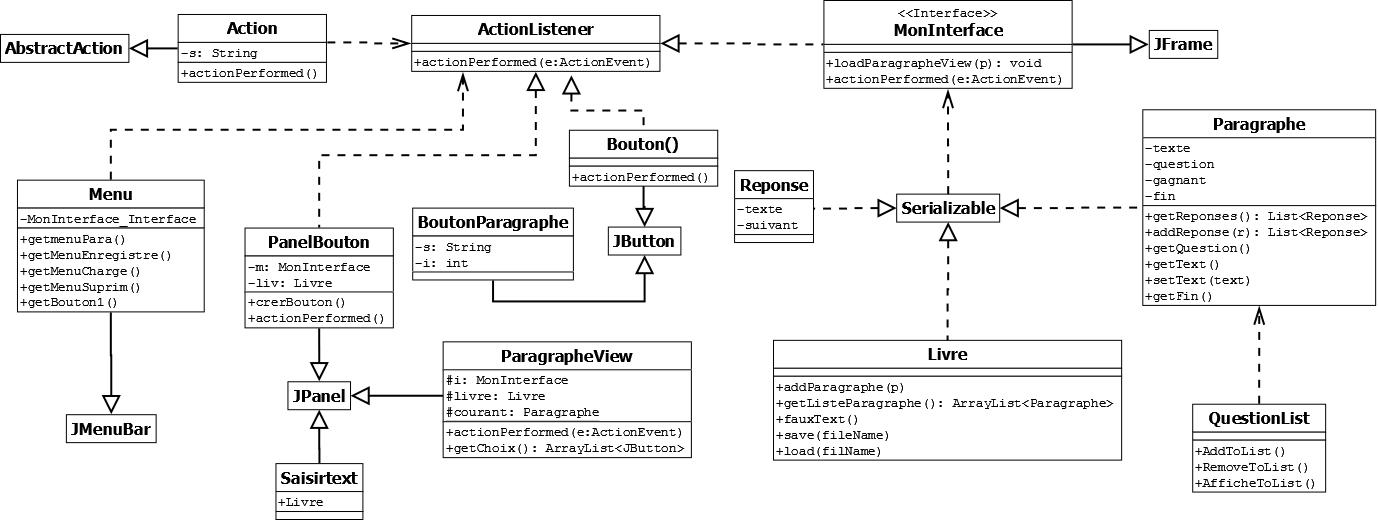
\includegraphics[width=1\textwidth]{DiagrammeDeClasse.png} 
  \end{center}
  \caption{Diagramme de Classes}
  \label{fig:mon_image}
 \end{figure} 
\end{frame}{}
   

    \subsubsection{Fonctionnalités}
\begin{frame}{Fonctionnalités}
    MonInterface est l’interface (GUI) : contient le livre, permet de sauvegarder le livre courant (via un JButton), permet de savoir quel est le paragraphe en cours d’édition,permet d’avoir une représentation du paragraphe en cours d’édition, la représentation
    des choix.\\
    JButton : Chaque JButton permet de demander à la GUI de charger le Paragraphe et la ParagrapheView associés au choix cliqué.\\
    La Classe Livre : permet de charger, d’ajouter les paragraphes. Elle permet de charger et d’enregistrer un fichier.\\
\end{frame}
\begin{frame}{Fonctionnalités}
    • Charger(dans livre)est une méthode statique La Classe Paragraphe : permet de voir le paragraphe courant .\\
    La Classe ParagrapheView : permet de voir la représentation du paragraphe en cours d’édition.\\
    • La méthode loadParagrapheVIew(dans MonInterface) permet de charger la vue (ParagrapheView) d’un paragraphe, ce paragraphe devenant le paragraphe courant, l’ancien paragraphe courant est sauvegardé via sa ParagrapheView.\\
\end{frame}{}
%--------------------------------

%-------------------
\section{\textbf{Réalisation}}
\begin{frame}{Réalisation}
  \begin{figure}[ht]
    \begin{center}
        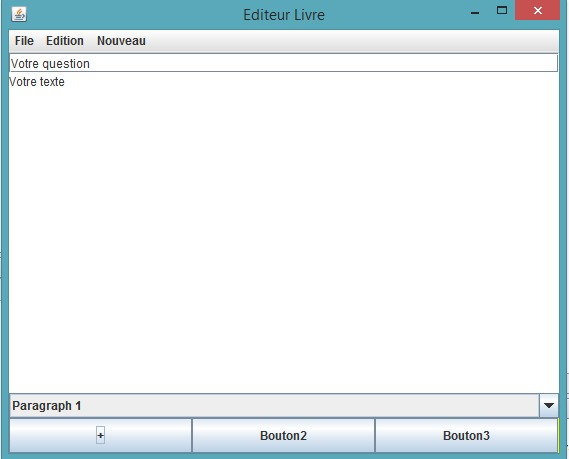
\includegraphics[width=0.6\textwidth]{1.jpg} 
     \end{center}
     \caption{ 2 Interface graphique}
     \label{fig:mon_image}
 \end{figure}
\end{frame}{}

\begin{frame}{Réalisation}
  \begin{figure}[ht]
    \begin{center}
        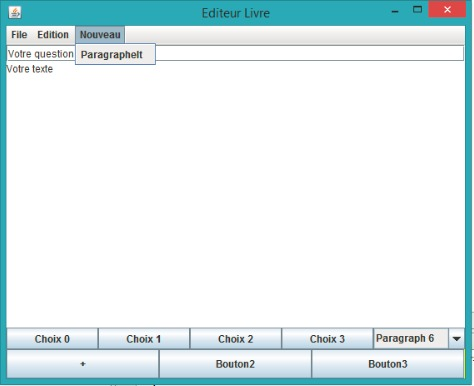
\includegraphics[width=0.6\textwidth]{3.jpg} 
     \end{center}
      \caption{ 3 Nouveau Paragraphe}
     \label{fig:mon_image}
  \end{figure}
\end{frame}{}

\begin{frame}{Réalisation}
  \begin{figure}[ht]
    \begin{center}
         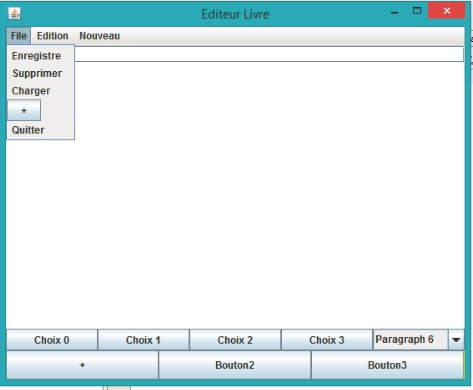
\includegraphics[width=0.6\textwidth]{2.jpg} 
     \end{center}
     \caption{ 4 elements du menu}
     \label{fig:mon_image}
 \end{figure}
\end{frame}{}



\begin{frame}{Réalisation}
   \begin{figure}[ht]
    \begin{center}
         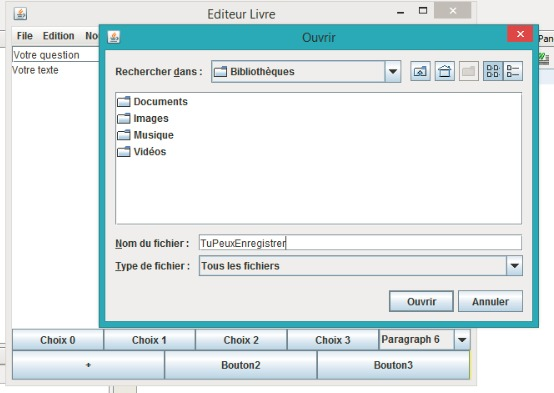
\includegraphics[width=0.8\textwidth]{4.jpg} 
     \end{center}
     \caption{ 5 Enregistrement et chargement d’un fichier}
     \label{fig:mon_image}
  \end{figure}
\end{frame}{}

\begin{frame}{Réalisation}
   \begin{figure}[ht]
    \begin{center}
         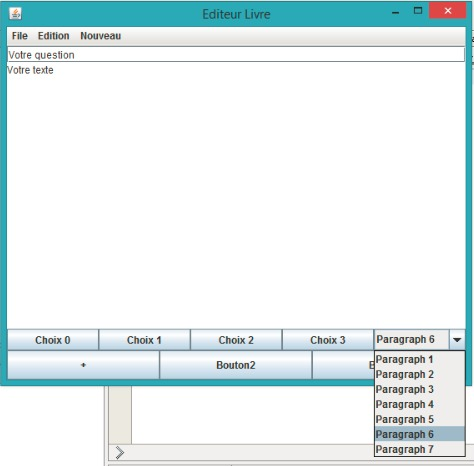
\includegraphics[width=0.6\textwidth]{5.jpg} 
     \end{center}
     \caption{ 6 Choix du paragraphe}
    \label{fig:mon_image}
  \end{figure}
\end{frame}{}

\begin{frame}{description des figures}
    \begin{itemize}
    \item La figure 2 représente l’interface principale de notre jeu.le joueur pourra écrire sa question et texte qui représente le paragraphe 1. On a trois menu : file, Edition et Nouveau.On a en bas une liste déroulante de tous les paragraphes qu’on a parcouru.Le bouton + permet d’ajouter un paragraphe.\\
    \item figure 3 le menu Nouveau on a ParagrapheTt qui permet d’ajouter un paragraphe.En bas on peut voir le nombre de choix,
    tout en choisissant les paragraphes dans l’ordre voulu.\\ 
    \item figure 4 représente les éléments de File et l’ordre de nos choix.
    On a : Enregistrer, Supprimer, Charger, un bouton + et Quitter.\\
   \item  figure 5 représente le chargement ou l’enregistrement d’un fichier.\\
   \item figure 6 On a sur la liste déroulante, tous les paragraphes créés. On peut choisir un paragraphe
    déjà choisi.
 \end{itemize}
\end{frame}{}
%------------------
\section{\textbf{Conclusion}}
 \begin{frame}{Conclusion}
     Ce projet a fait l’objet d’une expérience intéressante, meme si nous avions rencontrés quelques difficultés à le réaliser.\\
     Malgré tout, nous retiendrons de grandes leçons : l’importance des recherches, la valeur du temps dans la réalisation d’un programme etc.\\
     Tout n'est pas parfait certes,mais ce projet nous a permis d’améliorer nos connaissances et nos compétences dans le domaine de la conception logicielle .\\
    
 \end{frame}{}

\begin{frame}{}
  \begin{center}
      \textbf{MERCI DE VOTRE AIMABLE ATTENTION} 
  \end{center}     
\end{frame}


\end{document}